\documentclass[tikz,border=10pt]{standalone}
\usepackage{tikz}
\begin{document}
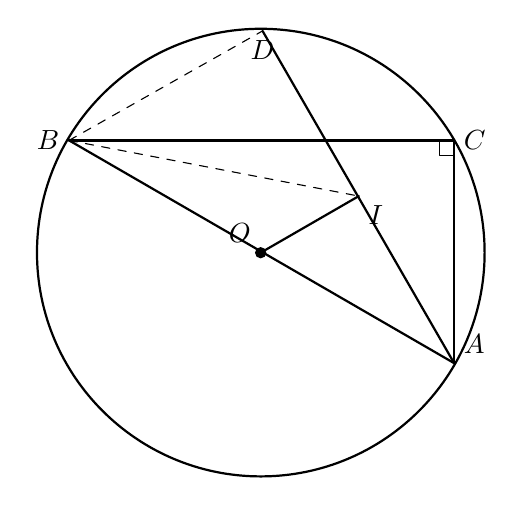
\begin{tikzpicture}[scale=0.012, line cap=round, line join=round]
% circle
\coordinate (O) at (273,245);
\coordinate (A) at (478,128);
\coordinate (B) at (70,364);
\coordinate (C) at (478,364);
\coordinate (D) at (275,480);
\coordinate (I) at (377,305);

\draw[thick] (273,245) circle (237);

\draw[thick] (B) -- (A);
\draw[thick] (A) -- (C);
\draw[thick] (B) -- (C);
\draw[thick] (A) -- (D);
\draw[thick] (O) -- (I);
\draw[dashed] (B) -- (I);
\draw[dashed] (B) -- (D);

% right angle mark at C
\draw (462,364) -- (462,348) -- (478,348);

\fill (O) circle (6);

\node[above left] at (O) {$O$};
\node[above right] at (A) {$A$};
\node[left] at (B) {$B$};
\node[right] at (C) {$C$};
\node[below] at (D) {$D$};
\node[below right] at (I) {$I$};
\end{tikzpicture}
\end{document}
